\chapter{Statistik und Wahrscheinlichkeit}
\chapterauthor{Rémy}
\section{Wiederholungen: Unter- \& Mittelstufe}
\subsection{Das Pascalsche Dreieck}
\subsection{Baumdiagramme}
\tikzstyle{level 1}=[level distance=3.5cm, sibling distance=3.5cm]
\tikzstyle{level 2}=[level distance=3.5cm, sibling distance=2cm]

% Define styles for bags and leafs
\tikzstyle{bag} = [text width=4em, text centered]
\tikzstyle{end} = [circle, minimum width=3pt,fill, inner sep=0pt]

% The sloped option gives rotated edge labels. Personally
% I find sloped labels a bit difficult to read. Remove the sloped options
% to get horizontal labels.
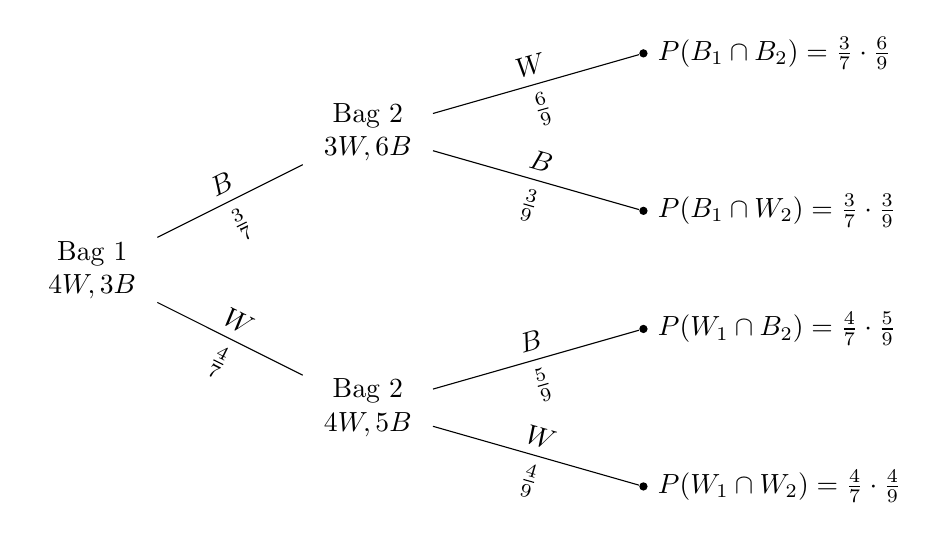
\begin{tikzpicture}[grow=right, sloped]
\node[bag] {Bag 1 $4W, 3B$}
    child {
        node[bag] {Bag 2 $4W, 5B$}
            child {
                node[end, label=right:
                    {$P(W_1\cap W_2)=\frac{4}{7}\cdot\frac{4}{9}$}] {}
                edge from parent
                node[above] {$W$}
                node[below]  {$\frac{4}{9}$}
            }
            child {
                node[end, label=right:
                    {$P(W_1\cap B_2)=\frac{4}{7}\cdot\frac{5}{9}$}] {}
                edge from parent
                node[above] {$B$}
                node[below]  {$\frac{5}{9}$}
            }
            edge from parent
            node[above] {$W$}
            node[below]  {$\frac{4}{7}$}
    }
    child {
        node[bag] {Bag 2 $3W, 6B$}
        child {
                node[end, label=right:
                    {$P(B_1\cap W_2)=\frac{3}{7}\cdot\frac{3}{9}$}] {}
                edge from parent
                node[above] {$B$}
                node[below]  {$\frac{3}{9}$}
            }
            child {
                node[end, label=right:
                    {$P(B_1\cap B_2)=\frac{3}{7}\cdot\frac{6}{9}$}] {}
                edge from parent
                node[above] {$W$}
                node[below]  {$\frac{6}{9}$}
            }
        edge from parent
            node[above] {$B$}
            node[below]  {$\frac{3}{7}$}
    };
\end{tikzpicture}

YUP, das ist Copy-Paste, don't blame me!
\subsubsection{Pfadregeln}
\section{Kombinatorik}
\subsection{Binomialkoeffizienten}
\begin{Definition}
  Der Binomialkoeffizient ist die Anzahl der $k$-elementigen Teilmengen einer $n$-elementigen Menge.
  $$ \left(\begin{array}{c} n \\ k \end{array}\right) = \dfrac{n!}{(n-k)!k!} \text{\qquad (gesprochen "n über k") }$$
\end{Definition}
\begin{Bemerkung}
  Anschaulich entspricht das den Möglichkeiten, genau $n$ bestimmte Kugeln zu ziehen, wobei die gezogenen Kugeln nicht zurückgelegt werden, und die Reihenfolge, in der sie gezogen wurden, nicht beachtet werden.
\end{Bemerkung}
\begin{Bemerkung}
  Die gefundenen Werte entsprechen den Vorfaktoren, die man für das $k$te Element aus der $n$ten Reihe aus dem Pascalschen Dreieck ablesen kann.\\
  Das bedeutet, dass Potenzen von Binomen auch über Binomialkoeffizienten darstellbar sind:
  $$(a+b)^n = \sum_{k=0}^n \left(\begin{array}{c} n \\ k \end{array}\right) a^{n-k}b^{k}$$
\end{Bemerkung}

\begin{Bemerkung}
  Da die Fakultät ($!$) nicht für negative Zahlen definiert ist, gilt die obige Definition nur für $0 \leq k \leq n$.
\end{Bemerkung}

\begin{GTR-Tipp}

\end{GTR-Tipp}

\subsection{Kombinatorik}
\begin{Theorem}
  Kombinatorik bezeichnet die Anzahl der Möglichkeiten der Anordnung von $k$ Elementen auf $n$ Stellen.\\
  Es werden 2 Fälle unterschieden:\\
  \begin{itemize}
    \item Die Reihenfolge der Elemente wird berücksichtigt:
          $$n(n-1)(n-2)...(n-(k-1))$$
    \item Die Reihenfolge der Elemente wird \textbf{nicht} berücksichtigt:
          $$\left(\begin{array}{c} n \\ k \end{array}\right)$$
  \end{itemize}
\end{Theorem}
\begin{Bemerkung}
  Auch hier gilt die Einschränkung $0 \leq k \leq n$. Diese ist sinnvoll, denn es ist nicht möglich, eine $k$-elementige Teilmenge einer $n$-elementigen Menge zu nehmen. Deshalb gilt:
  $$\text{Anzahl Möglichkeiten\,} = 0 \text{\qquad für \:} n \leq k $$
\end{Bemerkung}
\begin{Beweis}
  Es handelt sich hier eher um eine logische Begründung:\\
  \begin{itemize}
    \item Reihenfolge berücksichtigt:\\
    1. Auswahl: $n$ Möglichkeiten\\
    2. Auswahl: $n-1$ Möglichkeiten\\
    ..\\
    $k$-te Auswahl: $n-(k-1)$ Möglichkeiten\\
    $$\Rightarrow \text{\quad Möglichkeiten insgesamt:\, }  n(n-1)(n-2)...(n-(k-1))$$
    \item Reihenfolge \textbf{nicht} berücksichtigt:\\
    1. Auswahl: $n$ Möglichkeiten, 1 mögliche Permutation\\
    1. Auswahl: $n-1$ Möglichkeiten, 2 mögliche Permutationen\\
    ..\\
    $k$-te Auswahl: $n-(k-1)$ Möglichkeiten, $k$ mögliche Permutationen\\
    \begin{align*}
      \Rightarrow \text{\quad Möglichkeiten insgesamt:\, } & \dfrac{n(n-1)(n-2)...(n-(k-1))\text{\quad \} \small{1 neue Möglichkeit pro unterschiedlichem Fall}}}{1*2*...*(k-1)(k-2)k \text{ \quad \} \small{Anzahl der Wege, die zur selben Teilmenge führen}}}\\
      & = \dfrac{n(n-1)(n-2)...(n-(k-1))}{k!}\\
      & = \dfrac{n!}{(n-k)!k!}\\
      & = \left(\begin{array}{c} n \\ k \end{array}\right)
    \end{align*}

  \end{itemize}
\end{Beweis}
